\documentclass{letask}

\begin{document}
\begin{titlepage}
\center % Center everything on the page
 
%----------------------------------------------------------------------------------------
%	HEADING SECTIONS
%----------------------------------------------------------------------------------------

\textsc{\LARGE Московский\\[-0.2cm]Физико-Технический Институт\\[0.1cm]\large (государственный университет)}\\[1.5cm] % Name of your university/college
\textsc{\Large Кафедра общей физики}\\[0.1cm] % Major heading such as course name
\textsc{\large Лабораторная работа \textnumero  4.1.2}\\[0.5cm] % Minor heading such as course title

%----------------------------------------------------------------------------------------
%	TITLE SECTION
%----------------------------------------------------------------------------------------

\HRule
\\[0.4cm]
{ \huge \bfseries Моделирование оптических приборов\\[0.2cm]
и определение их увеличения}
\\[0.6cm] % Title of your document
\HRule
\\[1.5cm]


 
%----------------------------------------------------------------------------------------
%	AUTHOR SECTION
%----------------------------------------------------------------------------------------

	\begin{flushleft} \large
		\textsf{Студент}
		
		Маил \textsc{Мамедов} \\[-0.15cm]
		 группа Б01-006
	\end{flushleft}


\begin{bottompar}
	\begin{center}
		
\includegraphics[width = 80 mm]{logo.jpg}
	\end{center}
	{\large \today}

\end{bottompar}
\vfill % Fill the rest of the page with whitespace

\end{titlepage}

\textbf{Цель работы:} изучить модели зрительных труб (астрономической трубы Кеплера и земной трубы Галилея) и микроскопа, определить их увеличения.

\textbf{В работе используются:} оптическая скамья, набор линз, экран, осветитель со шкалой, зрительная труба, линейка.

\section{Теоретическая часть}
Оптические приборы, которые моделируются в данной работе: астрономическая труба Кеплера, земная труба Галилея и микроскоп.

Опишем каждую в общих чертах.

\subsection{Микроскоп}

Микроскоп состоит из двух собирающих систем линз — объектива
и окуляра, расположенных на расстоянии $l_{12}$ друг от друга в трубе, называемой тубусом. Предмет помещается на малом расстоянии перед передним фокусом объектива.


\begin{figure}[H]
\centering
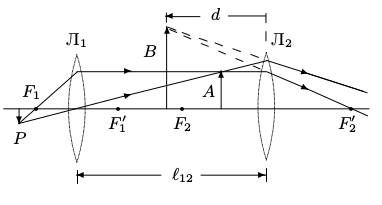
\includegraphics[width=0.6\lw]{1}
\caption{Ход лучей в микроскопе}
\end{figure}

Объектив Л$_1$ даёт действительное перевёрнутое увеличенное изображение $A$ предмета $P$, которое рассматривается через окуляр Л$_2$ , действующий как лупа. Мнимое изображение $B$, даваемое окуляром, располагается на некотором расстоянии $d$ от окуляра. Наводя микроскоп,
как и любой другой оптический прибор, на резкость, наблюдатель автоматически устанавливает такое расстояние $d$, которое удобно для аккомодации глаза.

В микроскопе фокусные расстояния $f_1$ и $f_2$ , а также оптический интервал $\Delta$ — положительны. Фокусное расстояние $f_M$ всей системы, а с
ним и увеличение $N_M$ — отрицательны, так что изображение, получаемое в микроскопе, — перевёрнутое (обратное).

\subsection{Зрительные трубы}

Зрительные трубы, основными элементами которых, как и в случае
микроскопа, являются объектив и окуляр, предназначены для наблюдения удалённых предметов.
Уменьшенное обратное изображение $A$
удалённого предмета, даваемое объективом, находится практически в
его фокальной плоскости. Мнимое изображение $B$, даваемое окуляром,
располагается на расстоянии $d$ от окуляра.
В теории зрительных труб для определённости считается, что глаз аккомодирован на бесконечность. При этом мнимое изображение $B$ должно располагаться в бесконечности, и, следовательно, промежуточное
изображение $A$ должно находиться в фокальной плоскости окуляра, а
задний фокус объектива должен быть совмещён с передним фокусом
окуляра.



Отношение фокусных расстояний может иметь
разный знак. Объективом зрительной трубы всегда является собирающая система, для которой переднее фокусное расстояние $f_1 > 0$. Окуляром трубы Кеплера является собирающая система,
переднее фокусное расстояние которой $f_2 > 0$, так что труба Кеплера даёт перевёрнутое изображение предмета. Окуляром трубы Галилея
, напротив, является рассеивающая система, переднее фокусное расстояние которой $f_2 < 0$, так что труба Галилея даёт прямое
изображение. Поэтому бытовые зрительные трубы, бинокли и т. д. делаются по схеме Галилея.

\begin{figure}[H]
\centering
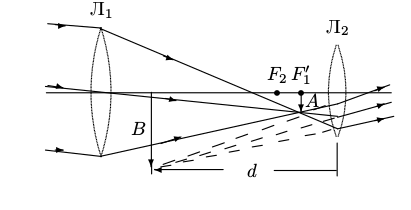
\includegraphics[width=0.6\lw]{2}
\caption{Ход лучей в зрительной трубе Кеплера}
\end{figure}

\begin{figure}[H]
\centering
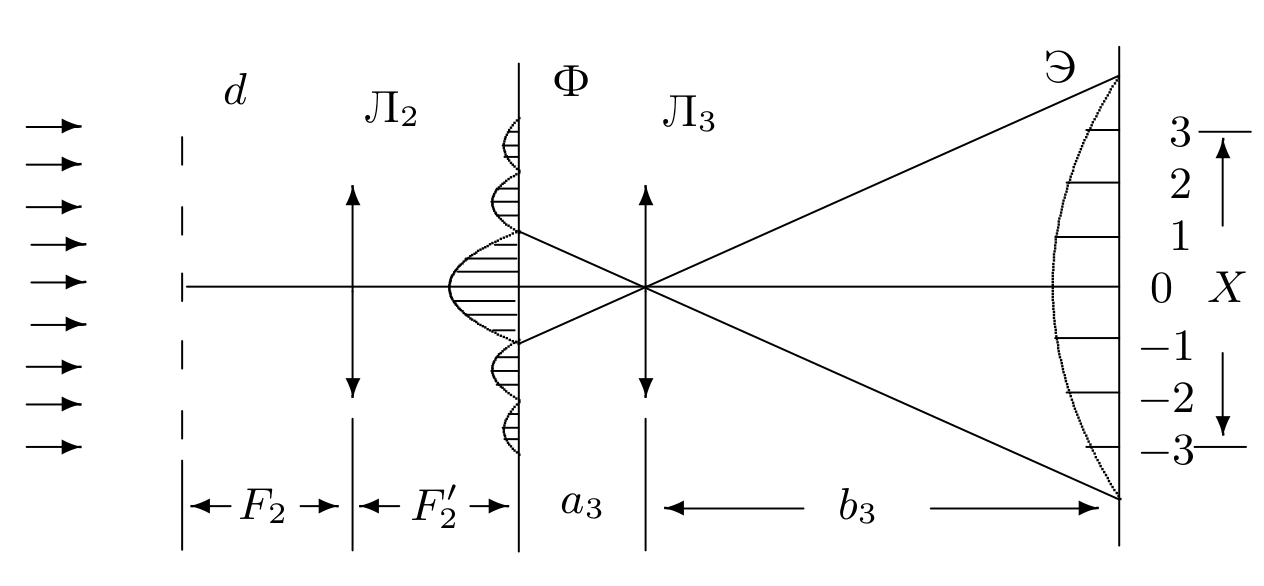
\includegraphics[width=0.6\lw]{3}
\caption{Ход лучей в зрительной трубе Галилея}
\end{figure}

\begin{figure}[H]
\centering
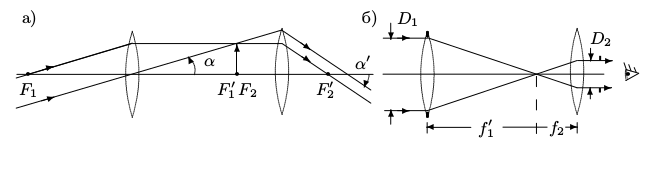
\includegraphics[width=0.8\lw]{4}
\caption{Ход лучей в телескопе}
\end{figure}

\section{Работа и обработка результатов}

\begin{enumerate}
\item Отцентрируем элементы оптической системы и определим приближенные значения фокусных расстояний линз:

\[f_1 = 9~\cm, \qquad f_2 = 11~\cm, \qquad f_3 = 21~\cm, \qquad f_4 = 28.5~\cm, \qquad f_5 = -10~\cm\]

\item Определим точные значения фокусных расстояний линз:

\[f_1 = 8.5~\cm, \qquad f_2 = 11~\cm, \qquad f_3 = 19.5~\cm, \qquad f_4 = 28~\cm \]

Для рассеивающей линзы по формуле $f = l - a_0$, измерив $l$:

\[l = 15.6~\cm, \quad a_0 = 25~\cm \quad \Rightarrow \quad f_5 = -9.4~\cm \]

\item Изучение телескопа Кеплера.

Определим размер изображения $h_1$ одного миллиметра шкалы осветителя в делениях
окулярной шкалы зрительной трубы без телескопа. $h_1 = k \tan{\alpha_1} \approx k \alpha_1$, где $k$~--~некоторый коэффициент, характеризующий увеличение зрительной трубы, $\alpha_1$~--~угловой размер изображения миллиметрового деления
шкалы осветителя, наблюдаемого через коллиматор.
\[h_1 = \dfrac{15}{20}~\text{дел}\]

Рассчитаем увеличение исследуемой модели телескопа по формуле:
\[N_T = -\dfrac{f_4}{f_2} = -\cfrac{28}{11} = -2.55 \pm 0.12\]

Определим размер изображения $h_2$ одного миллиметра шкалы осветителя в делениях окулярной шкалы зрительной трубы при наблюдении через телескоп. $h_2 = k \tan{\alpha_2} \approx k \alpha_2$, где $\alpha_2$~--~угловой размер изображения миллиметрового деления
шкалы осветителя, наблюдаемого через коллиматор.
\[h_2 = \dfrac{2.0}{1} = 2~\text{дел}\]

Рассчитаем увеличение исследуемой модели телескопа по формуле: 
\[N_T = \dfrac{\alpha_1}{\alpha_2} = -\dfrac{h_2}{h_1} = -\cfrac{2\cdot20}{15} = -2.67 \pm 0.22\]

Измерим диаметр оправы объектива и диаметр изображения этой оправы в окуляре:
\[D_1 = 3.7~\cm, \qquad D_2 = 1.4~\cm \]

Рассчитаем увеличение исследуемой модели телескопа по формуле:
\[N_T = - \dfrac{D_1}{D_2} = -2.64 \pm 0.20\]

\item Изучили модель трубы Галилея.

Аналогично:
\[h_1 = \dfrac{15}{20}~\text{дел}\]
\[h_2 = \dfrac{2.3}{1}~\text{дел}\]
\[N_T = -\dfrac{f_4}{f_5} = -\cfrac{28}{9.4} = -2.98 \pm 0.17\]
\[N_T = -\dfrac{\alpha_1}{\alpha_2}=-\dfrac{h_2}{h_1} = \cfrac{2.3\cdot 20}{15}  = -3.07 \pm 0.24\]

\item Создадим модель микроскопа с увеличением $N_M = 5$.

Рассчитали необходимый оптический интервал $\Delta$ и длину тубуса $l_{12}$ по формулам:
\[N_M = N_1 \cdot N_2 = - \dfrac{\Delta}{f_1} \cdot \dfrac{L}{f_2}\]
\[\Delta = l_{12} - f_1 - f_2 = 14.3~\cm\]
\[l_{12} = 39.8~\cm\]
Считаем $L=25~\cm$.
\[h_2 = \dfrac{3.2}{1}\] -- неточно, т.к. клетка полностью не влезала в видимое пространство

Измерили величину изображения $h_2$ миллиметрового деления предметной шкалы в делениях окулярной шкалы зрительной трубы и рассчитали увеличение по формуле 
\[N_M = - \dfrac{h_2}{h_1} \dfrac{L}{f_3} = \cfrac{3.2\cdot 20\cdot 25}{15\cdot 19.5} = 5.47 \pm 0.79\]
\end{enumerate}

\section{Вывод}
Полученные значения увеличений систем  достаточно неплохо согласуются между собой и различные методы дают очень близкие значения одних и тех же величин. Какие из методов оказались точнее видно из полученных ошибок в величинах.
\end{document}